\documentclass{beamer}
\usepackage{physics}
\usepackage{amsmath}
\usepackage{tikz}
\usepackage{mathdots}
\usepackage{yhmath}
\usepackage{cancel}
\usepackage{color}
\usepackage{siunitx}
\usepackage{array}
\usepackage{multirow}
\usepackage{amssymb}
\usepackage{textcomp, gensymb}
\usepackage{tabularx}
\usepackage{extarrows}
\usepackage{booktabs}
\usetikzlibrary{fadings}
\usetikzlibrary{patterns}
\usetikzlibrary{shadows.blur}
\usetikzlibrary{shapes}
\usepackage[style=verbose,backend=bibtex]{biblatex}
\addbibresource{arpes.bib}
\addbibresource{green.bib}
\usepackage{listings}
\usepackage{hyperref}

\newcommand{\pair}[1]{\langle #1 \rangle}
\DeclareMathOperator{\ee}{e}
\DeclareMathOperator{\ii}{i}

\newcommand{\concept}[1]{\textbf{#1}}

%Information to be included in the title page:
\title{Effective theories}
\author{Jinyuan Wu}

\usetheme{Madrid}

\begin{document}

\frame{\titlepage}

\begin{frame}
\frametitle{Effective theories}

\begin{itemize}
    \item Particle physicists and cosmologists come up with weird ideas to explain the world \dots
    \item but material scientists (or engineers) don't care. 
\end{itemize}

\textbf{Why?}

\begin{itemize}
    \item A phenomenon can be well described by a theory that \emph{fits its scale}
    \item \concept{Effective theory}
\end{itemize}

\end{frame}

\begin{frame}
\frametitle{Example 1}

We can use quantum theories to predict the behavior of electrons \dots%
\footnote{
    Picture from \href{https://en.wikipedia.org/wiki/Atomic\_orbital\#/media/File:Neon\_orbitals.png}{Wikipedia}.
}

\begin{center}
    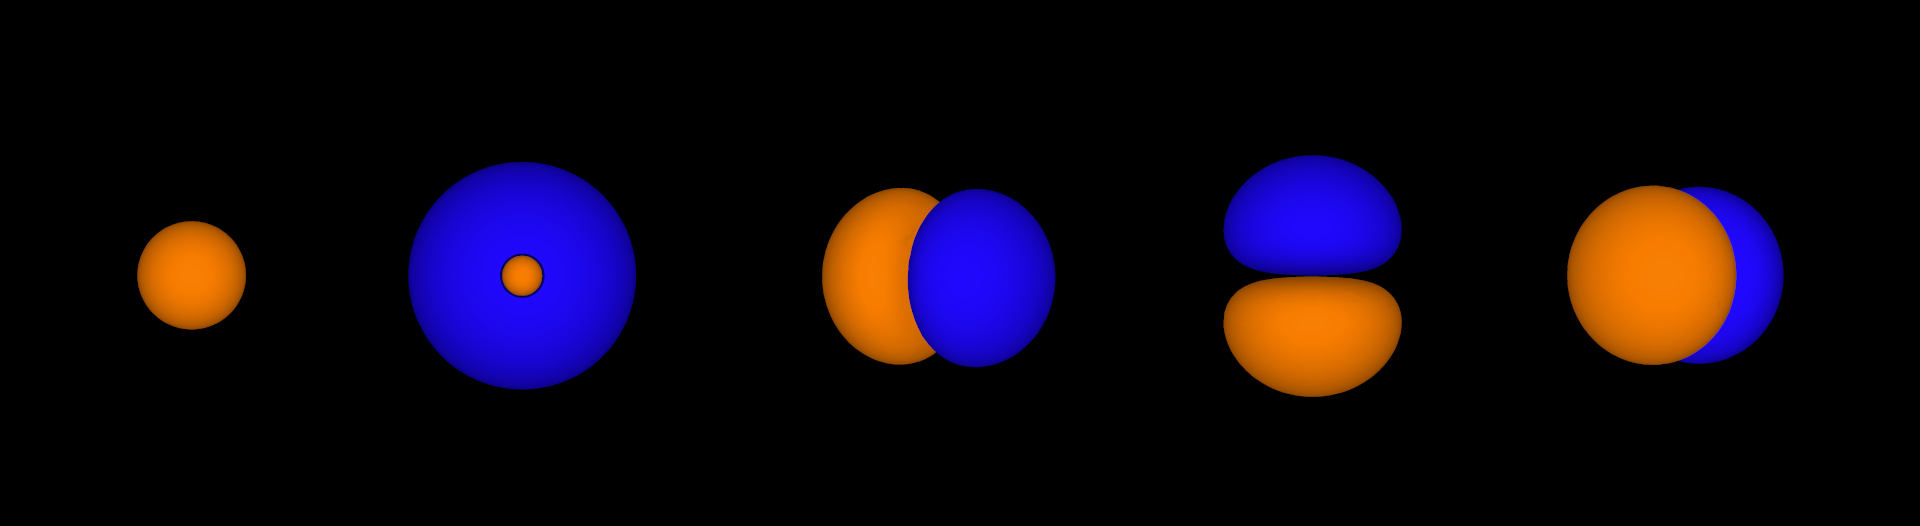
\includegraphics[width=0.5\textwidth]{newtonian/Neon_orbitals.png}
\end{center}

But the dynamics of molecule doesn't need full information concerning this:
Atoms are seen as balls without inner structures.\footnote{
    Picture from another \href{https://en.wikipedia.org/wiki/File:A\_molecular\_dynamics\_simulation\_of\_argon\_gas.webm}{Wikipedia page}.
}

\begin{center}
    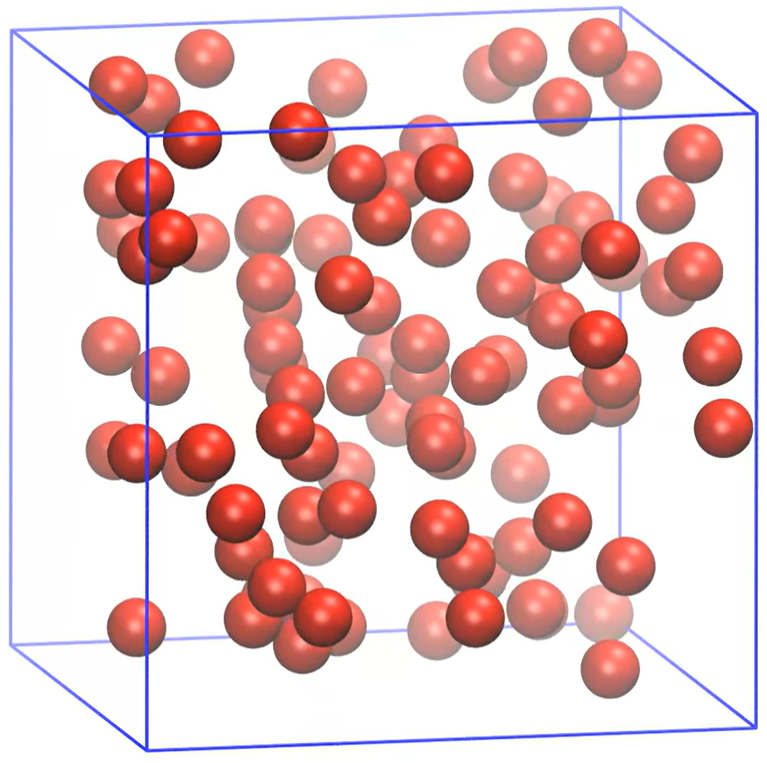
\includegraphics[width=0.3\textwidth]{newtonian/wiki-md.PNG}
\end{center}

\end{frame}

\begin{frame}
\frametitle{Example 2}

Electrons repulse each other -- Coulomb interaction\footnote{
    Picture from 
    \href{https://en.wikipedia.org/wiki/Coulomb\%27s\_law\#/media/File:CoulombsLaw.svg}{Wikipedia}.
}   

\begin{center}
    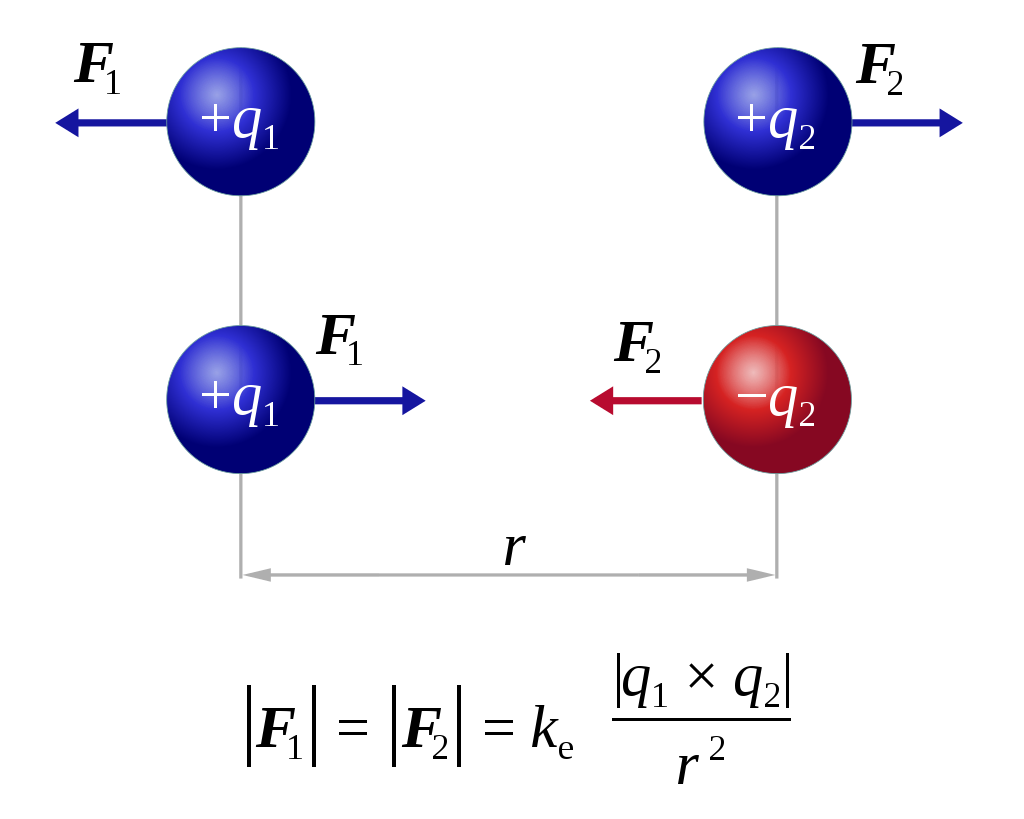
\includegraphics[width=0.3\textwidth]{ab-initio/CoulombsLaw.png}
\end{center}

But do you know this actually arises from changing photons (i.e. smallest unit of light)?

\begin{center}
    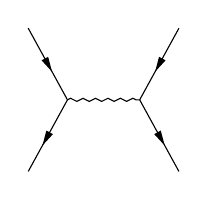
\begin{tikzpicture}[x=0.75pt,y=0.75pt,yscale=-0.6,xscale=0.6]
    %uncomment if require: \path (0,300); %set diagram left start at 0, and has height of 300
    
    %Straight Lines [id:da8755413231380609] 
    \draw    (314,106) -- (282.5,163.5) ;
    \draw [shift={(294.89,140.89)}, rotate = 298.72] [fill={rgb, 255:red, 0; green, 0; blue, 0 }  ][line width=0.08]  [draw opacity=0] (12,-3) -- (0,0) -- (12,3) -- cycle    ;
    %Straight Lines [id:da4411140816653467] 
    \draw    (193,106) -- (224.5,163.5) ;
    \draw [shift={(212.11,140.89)}, rotate = 241.28] [fill={rgb, 255:red, 0; green, 0; blue, 0 }  ][line width=0.08]  [draw opacity=0] (12,-3) -- (0,0) -- (12,3) -- cycle    ;
    %Straight Lines [id:da8299726687921312] 
    \draw    (193,221) -- (224.5,163.5) ;
    \draw [shift={(204.43,200.14)}, rotate = 298.72] [fill={rgb, 255:red, 0; green, 0; blue, 0 }  ][line width=0.08]  [draw opacity=0] (12,-3) -- (0,0) -- (12,3) -- cycle    ;
    %Straight Lines [id:da04225223106224618] 
    \draw    (314,221) -- (282.5,163.5) ;
    \draw [shift={(302.57,200.14)}, rotate = 241.28] [fill={rgb, 255:red, 0; green, 0; blue, 0 }  ][line width=0.08]  [draw opacity=0] (12,-3) -- (0,0) -- (12,3) -- cycle    ;
    %Straight Lines [id:da7722008970962935] 
    \draw    (224.5,163.5) .. controls (226.17,161.83) and (227.83,161.83) .. (229.5,163.5) .. controls (231.17,165.17) and (232.83,165.17) .. (234.5,163.5) .. controls (236.17,161.83) and (237.83,161.83) .. (239.5,163.5) .. controls (241.17,165.17) and (242.83,165.17) .. (244.5,163.5) .. controls (246.17,161.83) and (247.83,161.83) .. (249.5,163.5) .. controls (251.17,165.17) and (252.83,165.17) .. (254.5,163.5) .. controls (256.17,161.83) and (257.83,161.83) .. (259.5,163.5) .. controls (261.17,165.17) and (262.83,165.17) .. (264.5,163.5) .. controls (266.17,161.83) and (267.83,161.83) .. (269.5,163.5) .. controls (271.17,165.17) and (272.83,165.17) .. (274.5,163.5) .. controls (276.17,161.83) and (277.83,161.83) .. (279.5,163.5) -- (282.5,163.5) -- (282.5,163.5) ;
    
    
    
    
    \end{tikzpicture}
    
\end{center}

\end{frame}

\begin{frame}
\frametitle{Effective theories are everywhere}

\begin{itemize}
    \item Molecular dynamics is an effective theory of quantum mechanics.
    \item Coulomb interaction is an effective theory of quantum electrodynamics.
    \item \dots
\end{itemize}

A ``complete'' theory can also be an effective theory

General relativity  

\end{frame}


\begin{frame}
\frametitle{Conclusion}

\begin{itemize}
    \item A theory has 
\end{itemize}    

\end{frame}

\end{document}